% Created 2024-04-25 Thu 13:55
% Intended LaTeX compiler: pdflatex
\documentclass[smaller]{beamer}\usepackage{listings}
\usepackage{color}
\usepackage{amsmath}
\usepackage{array}
\usepackage[T1]{fontenc}
\usepackage{natbib}
\lstset{
keywordstyle=\color{blue},
commentstyle=\color{red},stringstyle=\color[rgb]{0,.5,0},
literate={~}{$\sim$}{1},
basicstyle=\ttfamily\small,
columns=fullflexible,
breaklines=true,
breakatwhitespace=false,
numbers=left,
numberstyle=\ttfamily\tiny\color{gray},
stepnumber=1,
numbersep=10pt,
backgroundcolor=\color{white},
tabsize=4,
keepspaces=true,
showspaces=false,
showstringspaces=false,
xleftmargin=.23in,
frame=single,
basewidth={0.5em,0.4em},
}
\usepackage{natbib, dsfont, pgfpages, tikz,amssymb, amsmath,xcolor}
\bibliographystyle{abbrvnat}
\setbeamertemplate{footline}[frame number]
\beamertemplatenavigationsymbolsempty
\usepackage{appendixnumberbeamer}
\setbeamercolor{gray}{bg=white!90!black}
\setbeamertemplate{itemize items}{$\circ$}
\lstset{basicstyle=\ttfamily\footnotesize}
\RequirePackage{fancyvrb}
\DefineVerbatimEnvironment{verbatim}{Verbatim}{fontsize=\footnotesize}
\definecolor{bblue}{rgb}{0.2,0.2,0.7}
\newcommand{\E}{{\ensuremath{\mathop{{\mathbb{E}}}}}}
\newcommand{\R}{\mathbb{R}}
\newcommand{\N}{\mathbb{N}}
\newcommand{\blank}{\makebox[1ex]{\textbf{$\cdot$}}}
\newcommand\independent{\protect\mathpalette{\protect\independenT}{\perp}}
\def\independenT#1#2{\mathrel{\rlap{$#1#2$}\mkern2mu{#1#2}}}
\renewcommand{\phi}{\varphi}
\renewcommand{\epsilon}{\varepsilon}
\newcommand*\diff{\mathop{}\!\mathrm{d}}
\newcommand{\weakly}{\rightsquigarrow}
\newcommand\smallO{\textit{o}}
\newcommand\bigO{\textit{O}}
\newcommand{\midd}{\; \middle|\;}
\newcommand{\1}{\mathds{1}}
\usepackage{ifthen} %% Empirical process with default argument
\newcommand{\G}[2][n]{{\ensuremath{\mathbb{G}_{#1}}{\left[#2\right]}}}
\DeclareMathOperator*{\argmin}{\arg\!\min}
\DeclareMathOperator*{\argmax}{\arg\!\max}
\newcommand{\V}{\mathrm{Var}} % variance
\newcommand{\eqd}{\stackrel{d}{=}} % equality in distribution
\newcommand{\arrow}[1]{\xrightarrow{\; {#1} \;}}
\newcommand{\arrowP}{\xrightarrow{\; P \;}} % convergence in probability
\newcommand{\KL}{\ensuremath{D_{\mathrm{KL}}}}
\newcommand{\leb}{\lambda} % the Lebesgue measure
\DeclareMathOperator{\TT}{\Psi} % target parameter
\newcommand{\empmeas}{\ensuremath{\mathbb{P}_n}} % empirical measure

\renewcommand*\familydefault{\sfdefault}
\itemsep2pt
\usepackage[utf8]{inputenc}
\usepackage[T1]{fontenc}
\usepackage{graphicx}
\usepackage{longtable}
\usepackage{wrapfig}
\usepackage{rotating}
\usepackage[normalem]{ulem}
\usepackage{amsmath}
\usepackage{amssymb}
\usepackage{capt-of}
\usepackage{hyperref}
\usetheme{default}
\author{Anders Munch}
\date{April 26, 2024}
\title{Motivating targeted learning}
\begin{document}

\maketitle

\begin{frame}[label={sec:orga6e9c25}]{A parameter of interest}
A target parameter is a functional
\begin{equation*}
  \Psi \colon \mathcal{P} \longrightarrow \R.
\end{equation*}

\vfill

Common case that
\begin{equation*}
  \Psi(P) = P{[ \phi(\blank; \nu(P)) ]}
  = \int \phi(x; \nu(P)) P(\diff x),
\end{equation*}
where $\nu$ is a function-valued nuisance parameter such as a conditional expectation or
a conditional probability.
\end{frame}


\begin{frame}[label={sec:orgadf46f6}]{A parameter of interest -- our setting}
\small

Population of women at their second birth \citep{wikkelso2014prediction}.

\vfill

The data consists of observations \( X = (Y, A, W) \), where \( Y \in \{0,1\}\) denotes PPH,
\( A \in \{0,1\} \) denotes planned c-section, and \( W \in \R^p \) is a vector
with information collected at the start of the second pregnancy, including
information from the first birth.

\vfill

Our parameter of interest is
\begin{align*}
  \Psi(P)
  & =
    \E_P
    {\left[
    \E_P{\left[ Y \mid A=1, W  \right]}
    - \E_P{\left[ Y \mid A=0, W  \right]}
    \right]}
  \\
  & = 
    P{[\nu(1, \blank; P) - \nu(0, \blank; P)]}    ,
\end{align*}
where
\begin{equation*}
  \nu(a, w; P) = \E_P{\left[ Y \mid A=a, W=w  \right]}.
\end{equation*}

\vfill

If \color{bblue}\(W\) includes all confounders of \(Y\) and \(A\)\color{black},
and there is \color{bblue}uniform positive probability of
treatment\color{black}, \(\Psi\)(P) can be interpreted as the average treatment
effect (ATE) of a planned c-section on PPH. This is known a the g-formula.
\end{frame}

\begin{frame}[label={sec:org575749a}]{Parametric modeling versus ML}
\small
\begin{block}{Parametric approach}
Fit a parametric model for \( \nu \) (e.g., logistic regression). Estimate
$\Psi$ with
\begin{equation*}
  \hat{\Psi}_n^{\text{glm}} =\empmeas{[\hat{\nu}_n^{\text{glm}}(1, \blank)- \hat{\nu}_n^{\text{glm}}(0,
    \blank)]}
  = \frac{1}{n}\sum_{i=1}^{n}
  \left\{
    \hat{\nu}_n^{\text{glm}}(1, W_i) - \hat{\nu}_n^{\text{glm}}(0, W_i)
  \right\}.
\end{equation*}
\end{block}


\begin{block}{Nonparametric (machine learning) approach}
Fit a machine learning algorithm to learn \( \nu \) (e.g., random forest).
Estimate $\Psi$ with
\begin{equation*}
  \hat{\Psi}_n^{\text{RF}} = \empmeas{[\hat{\nu}_n^{\text{RF}}(1, \blank)- \hat{\nu}_n^{\text{RF}}(0,
    \blank)]}
  = \frac{1}{n}\sum_{i=1}^{n}
  \left\{
    \hat{\nu}_n^{\text{RF}}(1, W_i) - \hat{\nu}_n^{\text{RF}}(0, W_i)
  \right\}.
\end{equation*}

\vspace{.4cm}


\begin{beamercolorbox}[rounded=true]{gray}
\centering \normalsize What would you prefer in our setting?
\end{beamercolorbox}
\end{block}
\end{frame}

\begin{frame}[label={sec:org9bee06b}]{Targeted estimators}
Semi-parametric efficiency theory tells us that an initial estimator can be
improved by adding an augmentation term:

\begin{equation*}
  \hat{\Psi}_n = \hat{\Psi}_n^{\text{RF}} + \empmeas{[\dot{\psi}(\blank, \hat{P}_n)]}.
\end{equation*}

\vfill

The function \(\dot{\psi}(\blank, P)\) is the \color{bblue}efficient influence
function \color{black} (aka \color{bblue}canonical gradient\color{black}) of
\(\Psi\).

\vfill

The term \(P{[\dot{\psi}(\blank, \hat{P}_n)]}\) can be interpreted as the
first order bias due to the estimation of \(\nu\) with \(\hat{\nu}_n^{\text{RF}}\), and we approximate this with \(\empmeas{[\dot{\psi}(\blank, \hat{P}_n)]}\).
\end{frame}

\begin{frame}[label={sec:orgcfecb75}]{Targeted estimators -- our setting}
\small

The EIF for our \(\Psi\) is well-known
\citep[e.g.,][]{kennedy2016semiparametric,kennedy2022semiparametric,hines2022demystifying}
and equals
\begin{align*}
  \dot{\psi}(X; P)
  & = \nu(W, 1; P) - \nu(W, 0;P)
    - \Psi(P)
  \\
  & \quad
    + \frac{A}{\pi(W;P)}(Y - \nu(W, 1; P))
    - \frac{1-A}{1-\pi(W;P)}(Y - \nu(W, 0;P)),
\end{align*}
where $\pi$ is the propensity score,
\begin{equation*}
  \pi(w; P) = P(A=1 \mid W=w).
\end{equation*}

\vfill

A targeted estimator of \(\Psi\) is then
\begin{align*}
  \hat{\Psi}_n= 
  \frac{1}{n}\sum_{i=1}^{n}
  \Big\{
  &
    \hat{\nu}_n^{\text{RF}}(1, W_i) - \hat{\nu}_n^{\text{RF}}(0, W_i)
    + \frac{A_i}{\hat{\pi}_n(W_i;P)}(Y_i - \nu(W_i, 1; P))
  \\
  & \quad
    - \frac{1-A_i}{1-\hat{\pi}_n(W_i;P)}(Y_i - \nu(W_i, 0;P))
    \Big\},
\end{align*}
where $\hat{\pi}_n$ is an estimator of $\pi$.
\end{frame}



\begin{frame}[label={sec:orgaf1fe4d},fragile]{Simulation study}
 \small

\begin{enumerate}
\item Generate a simulated data set of 800 individuals with 10 covariates.
\item Fit a ridge regression for the outcome using cross-validation to select
to penalty parameter
\item Use the fit from step 2 to and the g-formula to estimate the ATE. We refer to
this estimator as \texttt{naive}.
\item Fit another ridge regression for the propensity score using cross-validation
to select to penalty parameter
\item Use the efficient influence function and the estimators from step 2 and 4 to
target/debias the estimator calculated in step 3. We refer to this estimator
as \texttt{one-step}.
\end{enumerate}


\vfill

Repeat steps 1-5 1000 times to obtain 1000 samples of the \texttt{naive} estimator and
the \texttt{one-step} estimator.

\vfill

Examine performance of the two estimators by comparing these 1000 random samples
to the true ATE.
\end{frame}

\begin{frame}[label={sec:orge7bd75b}]{Result of simulation study}
\begin{center}
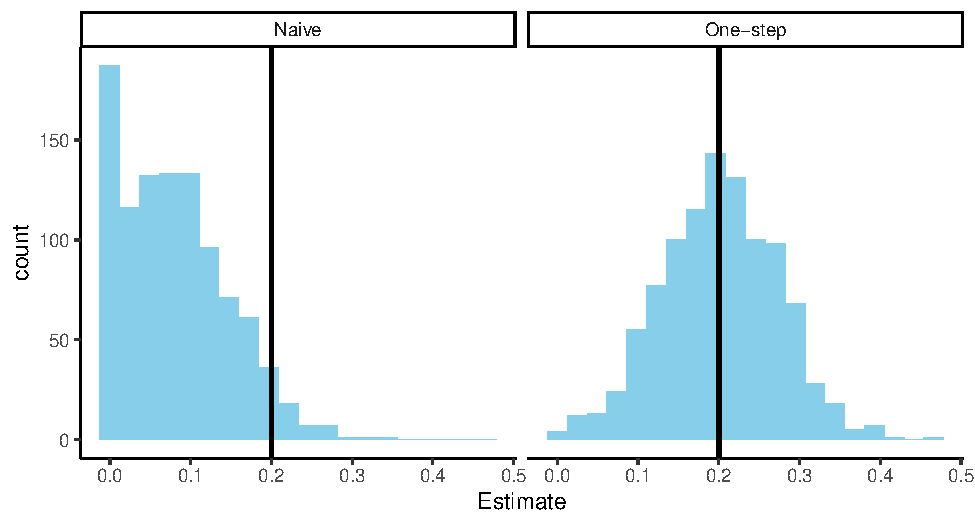
\includegraphics[width=.9\linewidth]{naive-vs-targeted.pdf}
\end{center}
\end{frame}

\begin{frame}[label={sec:org74f21f5},fragile]{Statistical inference}
 To quantify uncertainty we calculate confidence intervals. This procedure relies
on an estimate of the asymptotic variance of our estimator.

\vfill


\begin{block}{Naive ML approach}
\begin{itemize}
\item The use of cross-validation (and other data-adaptive algorithms) complicates
calculation of the asymptotic variance of the \texttt{naive} estimator.

\item Bootstrap is not feasible in practice (and works poorly with cross-validation)
\end{itemize}
\end{block}

\begin{block}{One step estimator}
\begin{itemize}
\item Closed form expression for the asymptotic variance which can be estimated
based on the models we have already fitted.
\end{itemize}
\end{block}
\end{frame}


\begin{frame}[label={sec:orgaeb7cc2}]{References}
\footnotesize \bibliography{bib.bib}
\end{frame}
\end{document}